\section{Introduction des Solutions}
\label{introSolutions}
	Le problème a résoudre, durant le stage, est d'améliorer la réactivité des réseaux pair à pair pour les MMOGs. La réactivité des protocoles pair à pair existants ne permet d'assurer la latence suffisante pour les application vidéoludique multijoueur. Blue Banana permet l'amélioration de la réactivité en rapatriant des données qui nous seront nécessaires dans un futur proche. Le travail effectué dans Blue Banana (cf \ref{BlueBanana}, page \pageref{BlueBanana}) s'intéresse à une partie du jeu bien définie, cette partie comprend les déplacements entre les zones denses. Durant le stage, il a donc fallu chercher des solutions qui permettraient d'améliorer le travail existant. Plusieurs pistes de solution ont été trouvées, deux de ces pistes ont été implémentées et testées. Les deux solutions implémentées, durant le stage, sont la mise en place d'un cache pour les zones denses de l'environnement, et la modification du rapatriement des données réalisé dans Blue Banana, pour les déplacements entre les zones denses.
\begin{table}[!h]
  \begin{center}
    \begin{tabular}{|c|c|}
      \hline
      Solution & Partie Améliorée \\
      \hline
      Introduction d'un cache  & Dans les zones denses \\
      Amélioration du préchargement & Entre les zones denses \\
      \hline
    \end{tabular}
  \end{center}
  \label{tab:config2}
  \caption{Tableau récapitulatif des solutions ajoutées durant le stage}
\end{table}
\par Dans la première solution, l'intérêt s'est porté sur une partie du jeu qui n'était pas étudiée dans Blue Banana. Le comportement des avatars dans les zones denses restait le même que dans Solipsis, nous avons donc décidé d'améliorer le fonctionnent dans ces zones denses. A l'intérieur de celles-ci, les joueurs se déplacent de façon désordonnée et bougent la plupart du temps dans un secteur restreint. L'utilisation d'un cache est alors apparu comme une solution d'amélioration. Le principe du cache est très simple, un nœud oubliait des voisins dont il pourrait avoir besoin dans un futur plus ou moins proche (en fonction de la mobilité dans le jeu), la mise en place du cache va permettre de garder un nombre \textit{N} de nœuds dans l'éventualité où le nœud revienne dans une zone où il est déjà venu (voir Schéma \ref{mouveDense}). Nous expliquerons les différentes solutions que nous avons testé pour le cache, et pourquoi celles que nous avons retenu fonctionnaient mieux.
        \begin{figure}[!h]
        \centering
        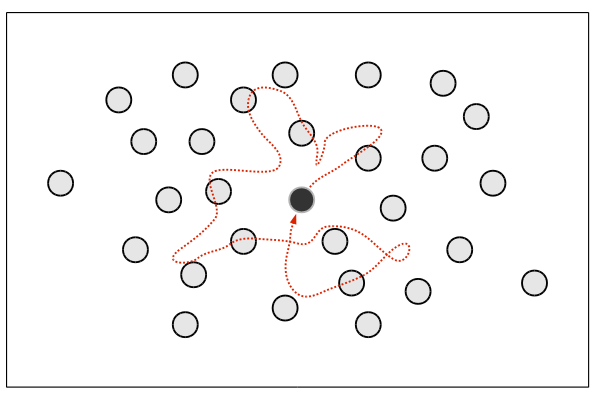
\includegraphics[scale=0.25]{./Ressources/Images/mouvementsZoneDense.png}\\
        \caption{Exemple d'une trajectoire d'un joueur dans une zone dense}
        \label{mouveDense}
        \end{figure}
\par La deuxième solution a consisté à modifier le préchargement des données réalisées dans Blue Banana, pour que celui-ci se fasse de manière plus fine. Les modifications que nous avons introduites doivent permettre d'économiser des messages et d'améliorer la cohérence de la topologie. Différentes techniques et algorithmes ont été testés, les plus importantes seront décrites et expliquées.
\par Les deux solutions mises en place permettent d'améliorer le travail qui avait déjà été effectué dans Blue Banana. Un des intérêts de nos solutions est qu'elles permettent d'améliorer une partie de l'environnement qui n'avait pas était traité (cache pour les zones denses), et d'améliorer un travail existant.


